\section{Results}
\label{sec:results}

\subsection{Physical range is part of the numerical problem}
\label{sec:range-result}
The CUDA diagnostic holds the query width at one and intervenes on the physical range supplied to attention--value multiplication. Cropping the wider execution from 1024 to 768 entries reproduces the shorter-reference output; padding the shorter execution to 1024 reproduces the wider output (Fig.~\ref{fig:extent}). Visible operands and probability prefixes agree in the captured case, and the added probabilities are zero. The bidirectional intervention supports the physical-range mechanism at that operator. It observes the complete attention--value output, rather than inferring equality from the eventual argmax.

\begin{figure*}[t]
 \centering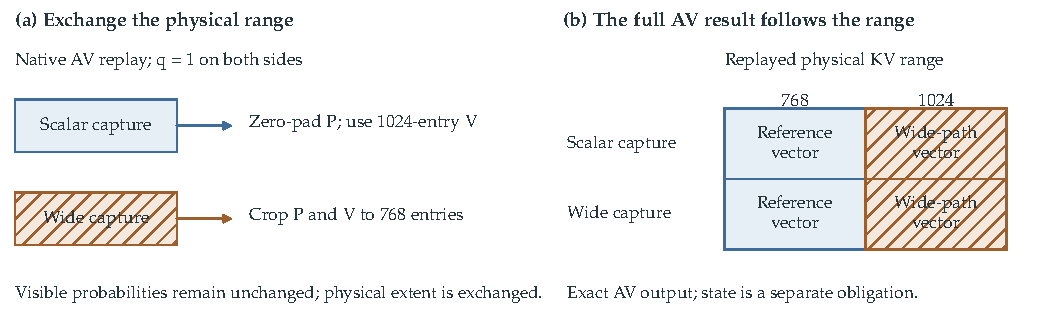
\includegraphics[width=\textwidth]{fig02_extent.pdf}
 \caption{A physical-range intervention changes the attention--value result. The captured CUDA comparison fixes a one-query consumer and tests 768- and 1024-entry physical ranges. Cropping and padding reproduce the respective reference outputs while retaining the visible operands. The observations concern the complete output of this operator; they do not measure KV-state equivalence or service time. The separate Vulkan study changes layout and dispatch together with range and is therefore a joint repair, not an isolated range intervention. Data and intervention identities are in the accompanying figure manifest.}
 \label{fig:extent}
\end{figure*}

At its tested boundaries, the 32B strong-control qualification passes comparisons of full 151,936-entry vocabulary vectors and active F16 KV across 64 layers. These observations complement the construction's conditional argument. The supplement identifies the coverage and retained records for the other profiles. Its CPU counterexamples show why the output and state obligations are necessary: matching argmax values can coexist with changed full vectors, serialized state and forced continuation.

\subsection{Independent groups improve on shared quantization}
\label{sec:strong-result}
Figure~\ref{fig:strong} shows the strongest direct service comparison for the execution organization. On the 32B target-only deployment, C/B is 0.984864, with a 95\% paired-root interval of [0.982148, 0.987721]. The corresponding reduction is 1.51\% [1.23\%, 1.79\%]. All 48 measured paired requests favor C, but the inferential unit is the 12 roots, not the 48 repeats.

\begin{figure*}[t]
 \centering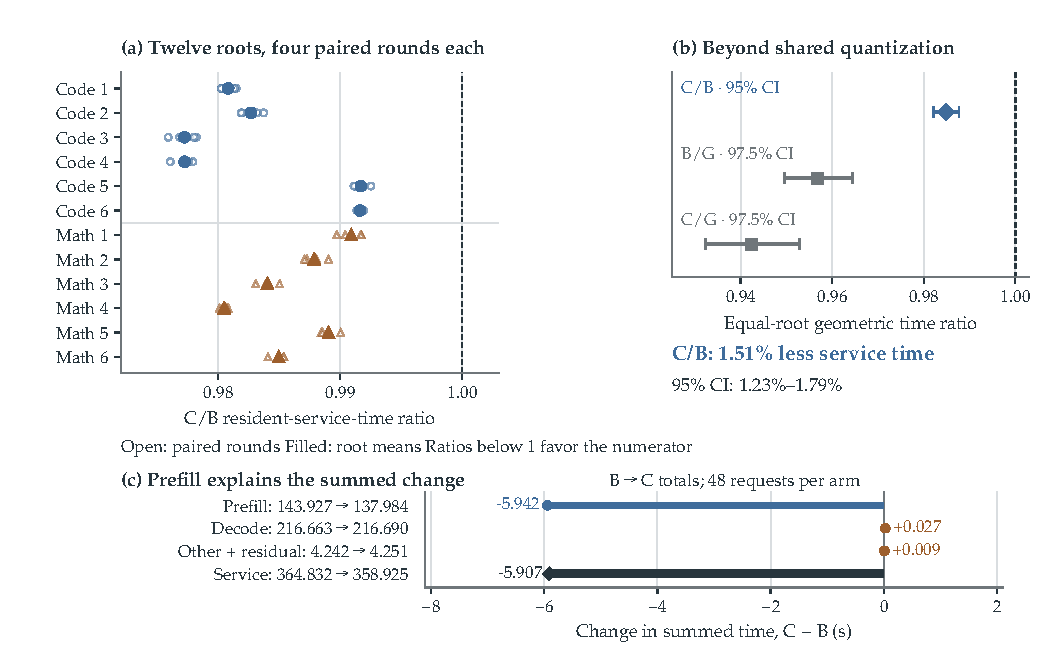
\includegraphics[width=\textwidth]{fig03_strong_baseline.pdf}
 \caption{The incremental service benefit beyond a strong same-contract control. A5000, Qwen3-32B-Q4\_K\_M, target-only generation, fixed whole-graph cuts. Root points average paired log ratios over four rounds. The primary C/B summary weights 12 roots equally and uses a 95\% paired-root interval stratified by coding and mathematics roots. Secondary B/G and C/G summaries use 97.5\% intervals. B shares activation quantization and invokes scalar backend projections; C schedules those scalar computations as independent channels. G is the weaker graph-level scalar loop. The resident timer includes reset and output ownership but excludes loading and diagnostic capture.}
 \label{fig:strong}
\end{figure*}

The weaker control explains why baseline choice matters. B/G is 0.956855 and C/G is 0.942372. Much of the advantage over G is already obtained by moving the scalar loop into the backend and sharing quantization. C/B isolates the remaining organization change. Across the 48 requests, B and C take 364.832 and 358.925\,s in total; their pooled ratio, 0.983809, differs from Eq.~\ref{eq:s3-estimand}. Prefill falls from 143.927 to 137.984\,s, while decode is effectively unchanged at 216.663 and 216.690\,s. This localization agrees with the opportunity to group known prompt rows. The result establishes a measurable compatibility-preserving increment in this deployment, without assigning draft-model benefits to it.

\subsection{Packing and local cuts have different opportunities}
\label{sec:factor-result}
The Q8 factorials fix the draft policy and cross cut placement with projection organization (Fig.~\ref{fig:factorial}). Packing reduces service by 1.64\% with \Simple{} and 1.56\% with \Local{} at 8B, and by 0.99\% and 0.80\% at 14B. Their backend-loop4 controls already share activation quantization, so these contrasts measure the remaining packed-group increment.

\begin{figure*}[t]
 \centering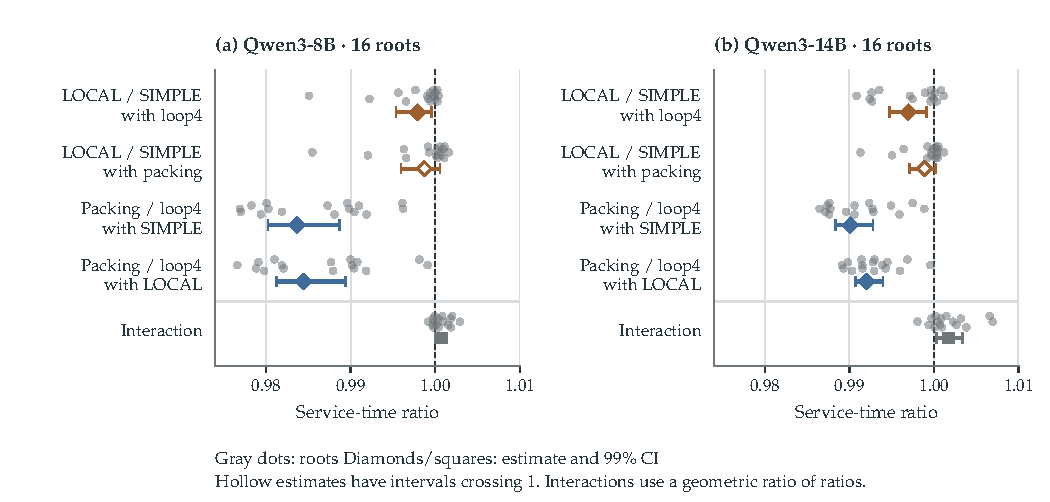
\includegraphics[width=\textwidth]{fig04_factorial.pdf}
 \caption{Separating the two execution changes. Balanced A5000 Q8 factorials fix draft prefill microbatch four and proposal count three. Faint points show individual root ratios; summary markers show ratios of total resident-service time with 99\% paired-root intervals from the five-comparison family. Projection contrasts hold cut placement fixed; cut contrasts hold projection fixed. The interaction summary is an equal-root geometric ratio of ratios. The two models share 16 task roots and are separate measurements. Intervals spanning one are visibly retained.}
 \label{fig:factorial}
\end{figure*}

Local cuts reduce service by 0.21\% and 0.30\% at fixed loop4. At fixed packing, the reductions are 0.13\% and 0.11\%, with both intervals containing zero reduction. The equal-root interactions are 1.000696 and 1.001703, indicating slight attenuation when both components are applied. At $k=3$, target verification has at most four queries, so it does not enter the multi-group Q8 packing route. Execution records place that route in prefill. The components consequently address different opportunities even within one request.

\subsection{Boundary geometry explains the local-cut results}
\label{sec:geometry-result}
In the natural 8B factorial, 20 of 2,224 logical verification cycles require an additional whole-graph split. \Simple{} uses 2,244 graphs and \Local{} 2,224 for the same target rows: just 0.899\% of cycles present that opportunity. The controlled B570 appends make the opportunity explicit (Fig.~\ref{fig:geometry}). A crossing starts one row before a physical boundary and forces the whole-graph split $1+(q-1)$, for $q=2,4,32$. Across capacities 1024 and 4096, local execution takes 20.34--44.68\% less append time in these cells. Matched inside controls take 0.43--3.74\% more time. Three paired observations per cell show repeat variation, not a workload confidence interval.

\begin{figure*}[t]
 \centering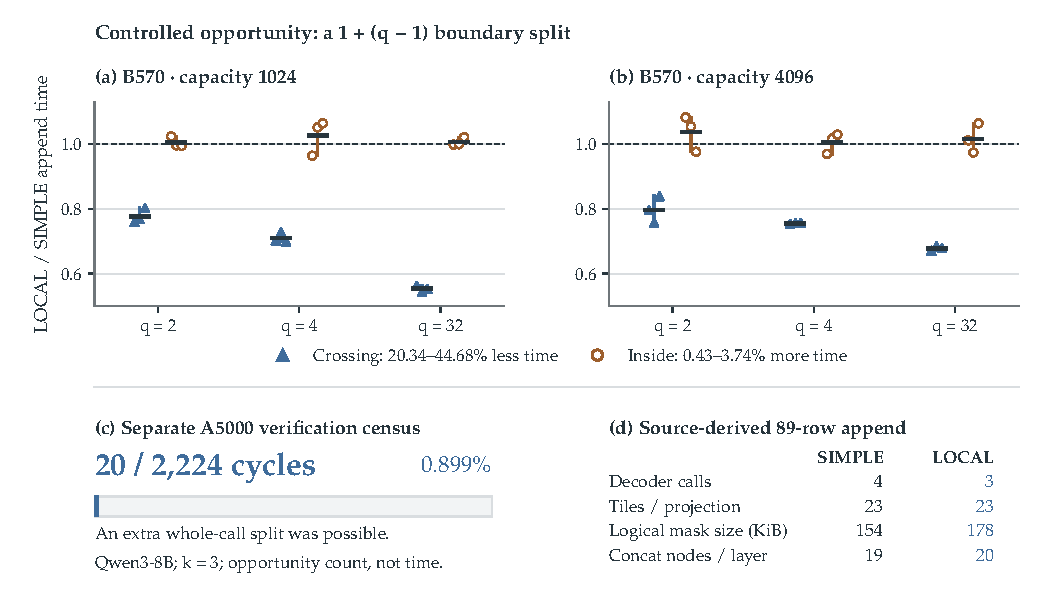
\includegraphics[width=\textwidth]{fig06_geometry.pdf}
 \caption{Local cuts help when they retain enough surrounding work. The opportunity count on A5000 is shown separately from B570 operation timings. B570 points compare \Local/\Simple{} append time at fixed $q$ and capacity; crossing triangles and inside circles use distinct shapes and fills. Ranges are the minimum and maximum of three paired repeats. The prepared-state timer includes binding, decode, synchronization and requested-output copying, and excludes state preparation. Capacity and prefix region change together between the two capacity panels. Earlier $16+16$ crossings, including reversals, are retained in the supplement.}
 \label{fig:geometry}
\end{figure*}

Crossing alone is not sufficient. Earlier $q=32$ cells with a $16+16$ whole-graph split include cases favoring \Simple{}. In the natural multi-turn pilot, the four paired episode ratios are 1.0997, 1.0024, 1.0886 and 0.9888 (Table~\ref{tab:natural}). Across the eight timed episodes, \Local{} takes 37.921\,s versus 36.385\,s for \Simple{}, a descriptive ratio of 1.04220. The pilot therefore provides no observed local-cut service improvement; two development conversations cannot establish a population ranking.

\begin{table}[t]
\centering\small
\caption{Natural multi-turn pilot: \Local/\Simple{} resident-service ratios. Packing and the request protocol are fixed. Rows are two rounds of each development episode, not four independent tasks. No confidence interval is inferred.}
\label{tab:natural}
\begin{tabular}{@{}lrr@{}}\toprule
Episode & Round 1 & Round 2\\\midrule
Development conversation A & 1.0997 & 1.0024\\
Development conversation B & 1.0886 & 0.9888\\\midrule
Pooled ratio & \multicolumn{2}{r}{1.04220}\\\bottomrule
\end{tabular}
\end{table}

The pilot's complete calls fall from 1,072 to 1,070. A separate source-derived plan for one proposed 89-row supplied-history append finds four versus three decoder calls but the same 23 ordered projection tiles. Fewer outer calls can therefore leave the principal arithmetic work unchanged. These observations identify limits on the natural-request opportunity: local placement avoids some graph fragmentation, while view construction, attention launches and concatenation remain real costs.

\subsection{Application gains are larger than the method increment}
\label{sec:application-result}
The complete Q8 speculative applications improve on all four target-only controls (Fig.~\ref{fig:application}). Against the fastest measured fixed M, \Local-packed D4 reduces resident service by 17.21\% for Qwen3-8B, 25.54\% for Qwen3-14B, and 11.52\% for Llama-8B. Their adjusted 99\% intervals are [11.17\%, 24.61\%], [18.21\%, 34.89\%], and [4.33\%, 20.95\%], respectively. These comparisons include the draft and the complete verification application. Against \Simple-loop4 with the same D4 policy, the corresponding increments are 2.01\%, 1.08\% and 1.56\%.

\begin{figure*}[t]
 \centering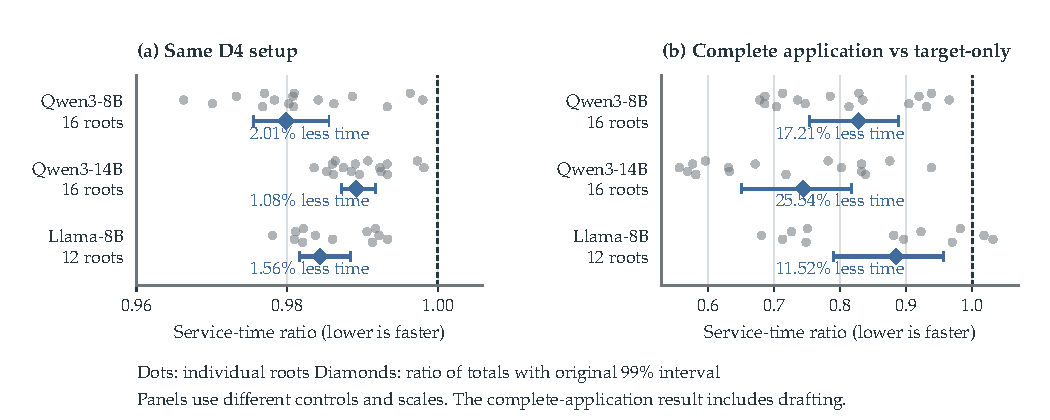
\includegraphics[width=\textwidth]{fig05_application.pdf}
 \caption{Application value and execution increment answer different questions. Panel (a) compares \Local-packed D4 with \Simple-loop4 D4 under the same draft policy; panel (b) compares it with the fastest measured fixed target-only control. Points retain root heterogeneity; summaries are ratios of total resident-service time with 99\% paired-root intervals. Qwen panels use the same 16 roots; Llama uses 12 separately selected roots. All fixed target-only comparisons are retained in the supplement, so choosing the fastest measured M does not replace the prespecified control family. The larger application reductions include speculative decoding.}
 \label{fig:application}
\end{figure*}

Initialization can change the decision. For the 14B request burst, worker time including loading, integrity checks and primers falls from 662.546\,s for W-P-M to 594.559\,s for \Local-packed D4. Llama's resident requests improve, yet its short worker workload favors target-only execution: the fastest M worker takes 355.730\,s versus 368.822\,s for \Local-packed D4. The earlier 32B panel instead favors ordinary grouped generation; grouped D4 takes about 14\% more resident time. A B570 pilot likewise favors target-only generation despite fewer target graphs in the speculative path. The supplement retains these complete cost accounts.

Wider execution also needs a workload distinction. A Windows RTX equal-work diagnostic makes one $q=8$ call 3.94--11.91\% cheaper than two $q=4$ calls from the same state with the same eight known tokens and requested outputs. In live generation, increasing proposals from $k=3$ to $k=7$ raises service time by 13.58--14.59\% across the four methods. For the same 11,472 emitted tokens, verification cycles fall from 3,504 to 2,296, but verified rows rise from 14,016 to 18,368 and draft proposals from 10,512 to 16,072. Avoiding launches does not repay the extra unconsumed work.

\subsection{A modern backend is a different engineering choice}
\label{sec:modern-result}
A recent upstream llama.cpp few-row implementation~\cite{llama_cpp_fewrow} provides a useful alternative. On one captured Qwen3-8B Q8 input with $K=N=4096$ and $q=8$, the ratio of upstream U to the extracted legacy packed Q8 operator B is 0.612924, with a 95\% paired-repeat interval [0.607906, 0.618665]. The 38.7\% reduction belongs to that operator comparison. U uses a different quantization and projection contract: 32,766 of 32,768 output bit patterns differ from the legacy reference. The preceding attempt to qualify U against the earlier strict CPU-round-to-nearest oracle for the upstream path failed and produced no timing under that oracle. The later comparison declares U's own contract instead.

This result favors considering a numerical migration when exact compatibility is unnecessary. It does not measure a complete default upstream backend: that backend's qualification and paired service timing have not been run. Two legacy-compatible extracted candidates also fail to improve the strong control, with complete-operator ratios 1.1264 and 1.0261 in their separate sessions. The available measurements compare operator choices; they leave the complete-backend service comparison open.
